\subsection{Diagramme de séquence}
Le diagramme de séquence a pour objectif de montrer les interactions entre les objets représentés par les classes du diagramme UML de la manière dont cela a été défini dans les use-case.
Nous présentons uniquement notre diagramme de séquence pour la gestion d'une demande.
En effet, nous n'avons pas eu le temps de concevoir les autres diagrammes de séquence.

\subsubsection{La gestion d'une demande}
L'acteur principal est le service des demandes. 
Celui-ci commence par vérifier l'existence du client via l'opération \texttt{checkExistence()}.
Cette opération prend le nom, le prénom et l'adresse en entrée, et renvoie un booléen.
Ce booléen permet alors soit de continuer les opérations, soit de créer un nouveau client.
Le nouveau client est créé via la méthode \texttt{new()} de personne.
Par la suite, le service enregistre le mode d'offre, le type de bien et le budget du client.
Ces informations sont sauvegardées par l'opération \texttt{savePreference()}.
Suite à cela, le système va chercher les classes standards respectant les critères du client via l'opération \texttt{getAllClasseStd()}.
L'employé ajoute les informations supplémentaires avec l'opération \texttt{saveInfosComplementaire()}.
Ces informations regroupent le choix du client sur plusieurs critères (présence d'un jardin, nombre de chambres, etc.).
L'opération \texttt{getListeBiens()} enregistre pour un client, selon ces critères et les classes standards qui lui sont associées, les biens disponibles.
Finalement, l'opération \texttt{updateList()} sert à peaufiner la liste générée à l'étape précédente.
Ce tri est dicté par le client selon ses premières impressions.\\

En réalisant ce diagramme de séquence, nous nous sommes rendus compte que la classe client n'est pas complète. Nous n'avions pas pensé que nous aurions besoin de champs indépendants pour les différents choix du client. Ces champs sont optionnels. Toutefois ils sont nécessaires pour conserver les choix du client dans le système d'information.\\

Un schéma représentant les interactions entre les classes est disponible à la figure \ref{fig:sequence} p.\pageref{fig:sequence}

\newpage
\begin{landscape}
	\begin{figure}[H]
		\centering
		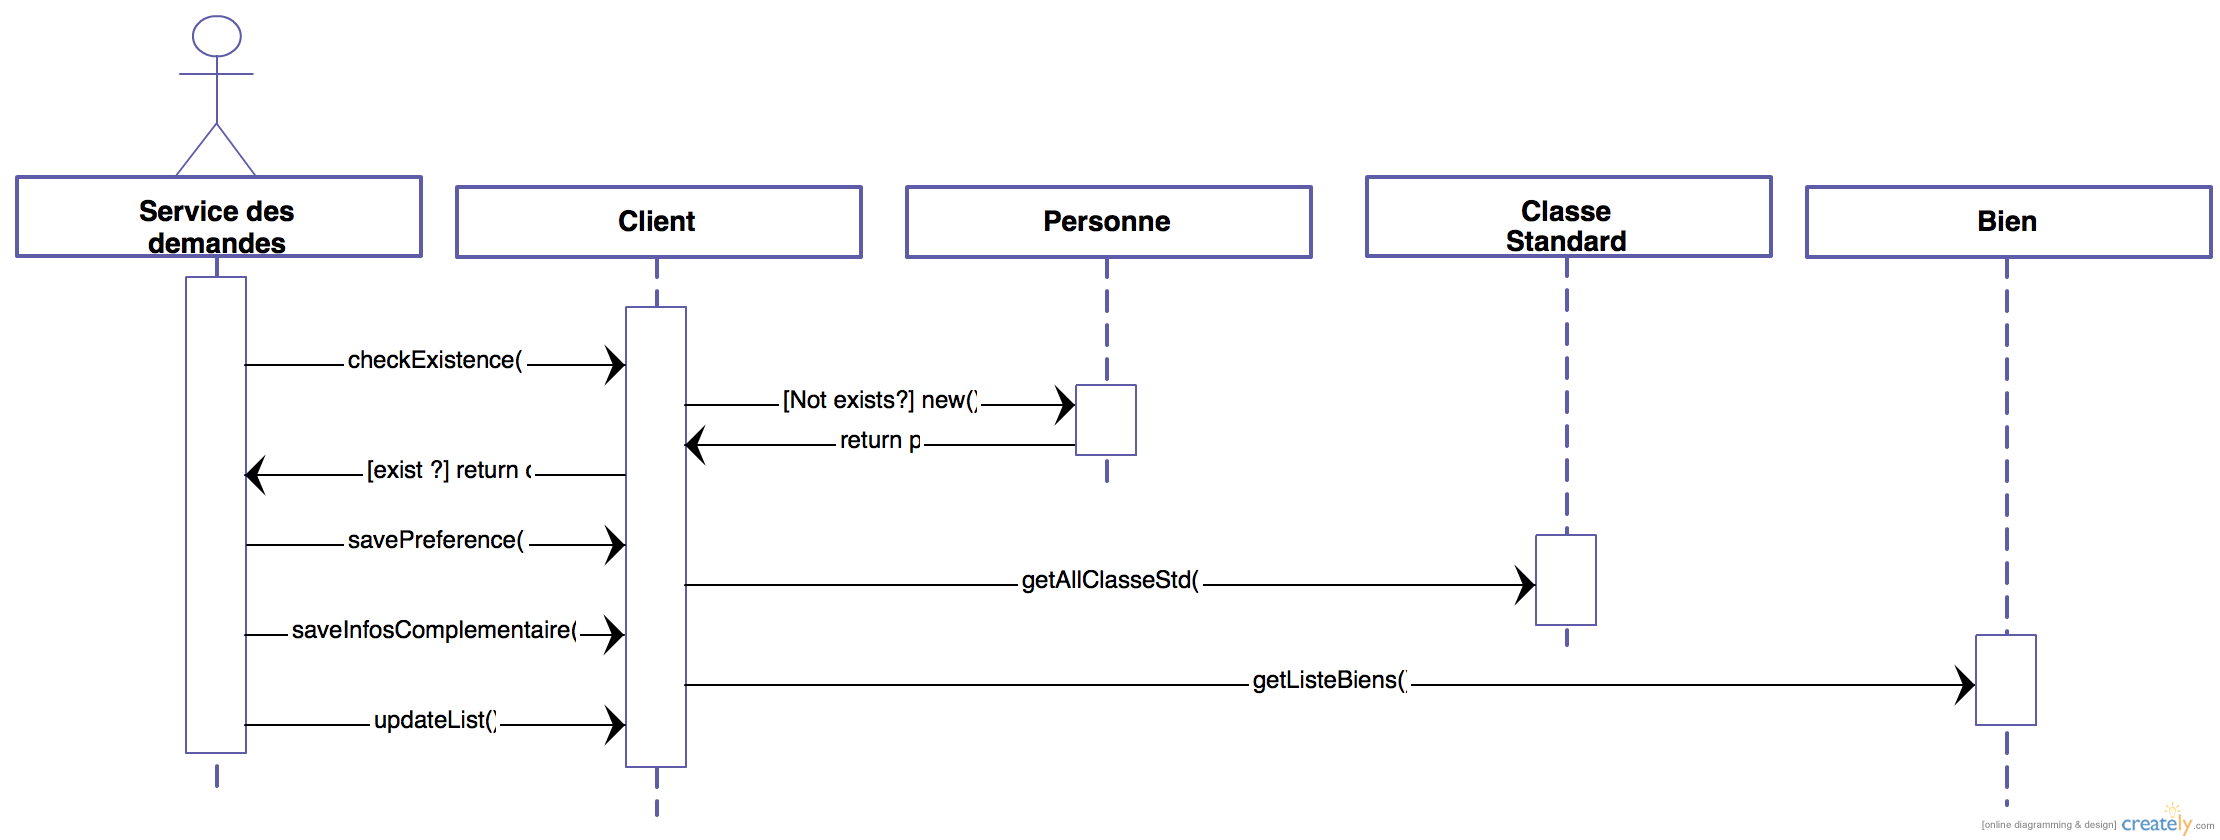
\includegraphics[width=23cm]{Sequence-DemandeBien.png}
		\caption{Diagramme de séquence - Gestion d'une demande}
		\label{fig:sequence}
	\end{figure}	 
\end{landscape}